% p16-commutativity-for-f-equals-apply-h-times-id.tex
%
% Source:   Carl A. Gunter and Dana S. Scott, "Semantic Domains" (1990).
%           ScottDomains/papers/Gunter Scott 1990.pdf
% Physical page: 16          Printed page: 15
% Section:  4.1 "Products" (the diagram is at the very top of printed page 15;
%           subsection 4.2 begins further down the same page).
% Unnamed in the paper - no figure number, no caption.
%
% Introducing sentence (verbatim, end of printed page 14):
%   "On the other hand, if curry(f) is uniquely determined by the diagram
%    above, then equation (1) follows immediately from the commutativity of
%    the following diagram:"
% and the line closing it, immediately below the diagram (printed page 15):
%   "for f = apply \circ (h \times id_E)."
%
% What the development uses it for: it is the converse direction of the
% equivalence between the uniqueness of curry(f) and equation (1),
% curry(apply \circ (h \times id_E)) = h. It is the diagram of physical
% page 15 with the mediating arrow taken to be an arbitrary h \times id
% rather than curry(f) \times id.
%
% The vertical arrow h \times id is the one the paper draws DASHED.
%
% Geometry measured from a 150 dpi render of physical page 16: D \times E and
% F are 147 px apart horizontally and (E \to F) \times E sits 148 px below
% D \times E - the same 2.5 by 2.5 cm as the diagram on physical page 15.
%
% Style contract (r0039) with the orchestrator-settled corrections, plus the
% "obj", "arrow" and "darrow" styles this commutative diagram needs (see
% p08-uniform-fixed-point-operator.tex for the note).

\documentclass[border=6pt]{standalone}
\usepackage{tikz}
\begin{document}
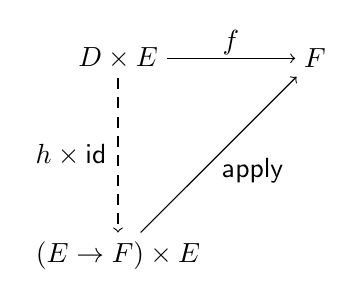
\begin{tikzpicture}[
  x=1cm, y=1cm,
  every node/.style={inner sep=1pt},
  open/.style={circle, draw, fill=white, minimum size=4pt, inner sep=0pt},
  solid/.style={circle, draw, fill=black, minimum size=5pt, inner sep=0pt},
  edge/.style={draw, line width=0.4pt},
  obj/.style={inner sep=3pt},
  arrow/.style={draw, line width=0.4pt, ->},
  darrow/.style={draw, line width=0.4pt, ->, dash pattern=on 4pt off 3pt}]

  \node[obj] (DE)  at (0.0, 2.5) {$D \times E$};
  \node[obj] (F)   at (2.5, 2.5) {$F$};
  \node[obj] (EFE) at (0.0, 0.0) {$(E \to F) \times E$};

  \draw[arrow]  (DE)  -- node[above] {$f$} (F);
  \draw[darrow] (DE)  -- node[left=3pt] {$h \times \mathsf{id}$} (EFE);
  \draw[arrow]  (EFE) -- node[below right] {$\mathsf{apply}$} (F);

\end{tikzpicture}
\end{document}
